% Created 2020-10-25 So 23:03
% Intended LaTeX compiler: pdflatex
\UseRawInputEncoding

\documentclass[11pt]{scrartcl}
\usepackage[utf8]{inputenc}
\usepackage[T1]{fontenc}
\usepackage[ngerman]{babel}
\usepackage{graphicx}
\usepackage{grffile}
\usepackage{longtable}
\usepackage{wrapfig}
\usepackage{rotating}
\usepackage[normalem]{ulem}
\usepackage{amsmath}
\usepackage{upgreek}
\usepackage{trfsigns}
\usepackage{textcomp}
\usepackage{amssymb}
\usepackage{capt-of}
\usepackage{MnSymbol}
\usepackage{mathtools}
\usepackage{setspace}
\usepackage{nicematrix}
\usepackage{empheq}
\usepackage{pdfpages}
% \usepackage{getlab}
\usepackage{listings}
\usepackage{pdfpages}
\usepackage[straightvoltages, european resistors, european inductors]{circuitikz}
\usetikzlibrary{arrows.meta}
\tikzset{FARROW/.style={arrows={-Triangle[angle=45:2.0mm]}}}
% \usepackage{varwidth}
\usepackage{hyperref}


\definecolor{darkspringgreen}{rgb}{0.09, 0.45, 0.27}    % Farbe für die Kommentare bei Listings
\lstset{
  language= Matlab,                     % Setzt die Sprache
  basicstyle=\scriptsize\ttfamily,     % Setzt den Standardstil
  % keywordstyle=\color{red}\bfseries,    % Setzt den Stil für Schlüsselwörter
  identifierstyle=\color{blue},        % Identifier bekommen keine gesonderte formatierung
  commentstyle=\color{darkspringgreen},        % Stil für Kommentare
  stringstyle=\ttfamily,             % Stil für Strings (gekennzeichnet mit "String")
  breaklines=true,             % Zeilen werden umgebrochen
  numbers=left,                 % Zeilennummern links
  numberstyle=\tiny,             % Stil für die Seitennummern
  frame=single,                 % Rahmen
  % backgroundcolor=\color{myGrey},     % Hintergrundfarbe
  % caption={Java-Code},             % Caption
  tabsize=2                % Größe der Tabulatoren
}



\newcommand{\GETHeader}[6]{%
  \begin{titlepage}
    \pagestyle{empty} \enlargethispage*{25cm}\samepage{
      \vspace*{-2.5cm}
      \begin{center}
        %
        \begin{tabular}[b]{lr}
          %
          \hspace*{-1.5cm}
          \begin{tabular}{p{3.8cm}}
            
\includegraphics[width=3.8cm]{./Figures/TUGraz}
          \end{tabular}
          %
          \hspace*{-1cm}
          %
          %
          \begin{tabular}{p{13.8cm}}
            \begin{flushright}
              \large
              Institut für Grundlagen und Theorie der Elektrotechnik\\
              ~\\
            \end{flushright}
          \end{tabular}
        \end{tabular}

        \vspace*{2.2cm}
        %
        \Huge {Elektrische Netzwerke und Mehrtore \\ Übung\\} %
        \vspace*{.5cm} \Large{ Wintersemester 2020\\}
        %
        \vspace*{1.5cm}

        \Huge{\textbf{#1}\\}

        %
        % \vspace*{0.8cm} \Large{Übungsdatum: {#2}\\}
        %
        \vspace*{1cm} \vfill
        %
        \Large{Gruppe: {#2}\\} \vspace*{0.5cm}%


        % \Large{Protokollführer(in): {#3}\\} \vspace*{1cm}

        \Large{Gruppenteilnehmer:\\} \vspace*{.1cm}
        % Name der beteiligten Studierenden
        \Large{#3} \vspace{1cm}
        %
        %
        \Large{Vortragende: #4\\} \vspace*{.1cm}   %\vspace*{1.5cm}
        % \Large{Betreuer(in): #6\\}
        \vspace*{1.5cm}
        %
        \Large{#5, am #6}
      \end{center}}%
    %
    \clearpage
  \end{titlepage}}








\begin{document}

\GETHeader                                                                              %  Bitte Ausfüllen!!!
% ----------------------------
{Protokoll Übung 5: \\ Frequenzbereich}                         %  Übungstitel
% ----------------------------
% {25. Mai 2020}                                                                  %  Übungsdatum
% ----------------------------
{04}                                                                   %  Gruppen-Nr.
% ----------------------------
% {Matthias Fottner}                                                                      % Name des Protokollführers oder der Protokollführerin
% ----------------------------
{
  \begin{center}
    \begin{minipage}{0.28\linewidth}
      1. Matthias Fottner\\
      2. David Keller\\
      3. Moritz Woltron
    \end{minipage}
  \end{center}
}
% ----------------------------
{Helena Grabner}                                                                     %  Laborleiter(in)
% {Übung 2}                                                               %  Betreuer(in)
% ----------------------------
{Graz}                                                                                  %  Ort der Protokollerstellung
{\today}                                                                %  Datum Protokollerstellung


\newcommand{\unit}[1]{\,\text{#1}}


\tableofcontents

\newpage


\allowdisplaybreaks

\setlength{\jot}{10pt}

\section{Zeichnen der beiden maßstabsgetreuen Zeigerdiagramme}
\label{sec:zeichnen-der-beiden}

Bei den Diagrammen \ref{fig:diagramm-spule} und \ref{fig:diagramm-kond} können bloß die absoluten Werte von $i_{L}=i_{R}$, $u_{R}$, $u_{L}$ und $u_{X}$ mit deren jeweiligen Phasenbeziehungen bestimmt werden. Eine genaue Bestimmung des Betrags von $\underline{i_{X,L}}$ bzw. $\underline{i_{X,C}}$ ist ohne weitere Bedingung nicht möglich. Allerdings muss dieser Zeiger um $\pm 90^{\circ}$ von $\underline{u_{X}}$ verschoben sein.

\subsection{bei angenommener Spule}
\label{sec:bei-angen-spule}
Die Spannungen wurden wie in Kapitel \ref{sec:skript-zu-spule}, Zeile 52 ersichtlich, mit dem Faktor $1,7$ skaliert. Dies gewährleistet die Darstellung von Strom und Spannung in einem Zeigerdiagramm.

\begin{figure}[!htb]
    \begin{center}
      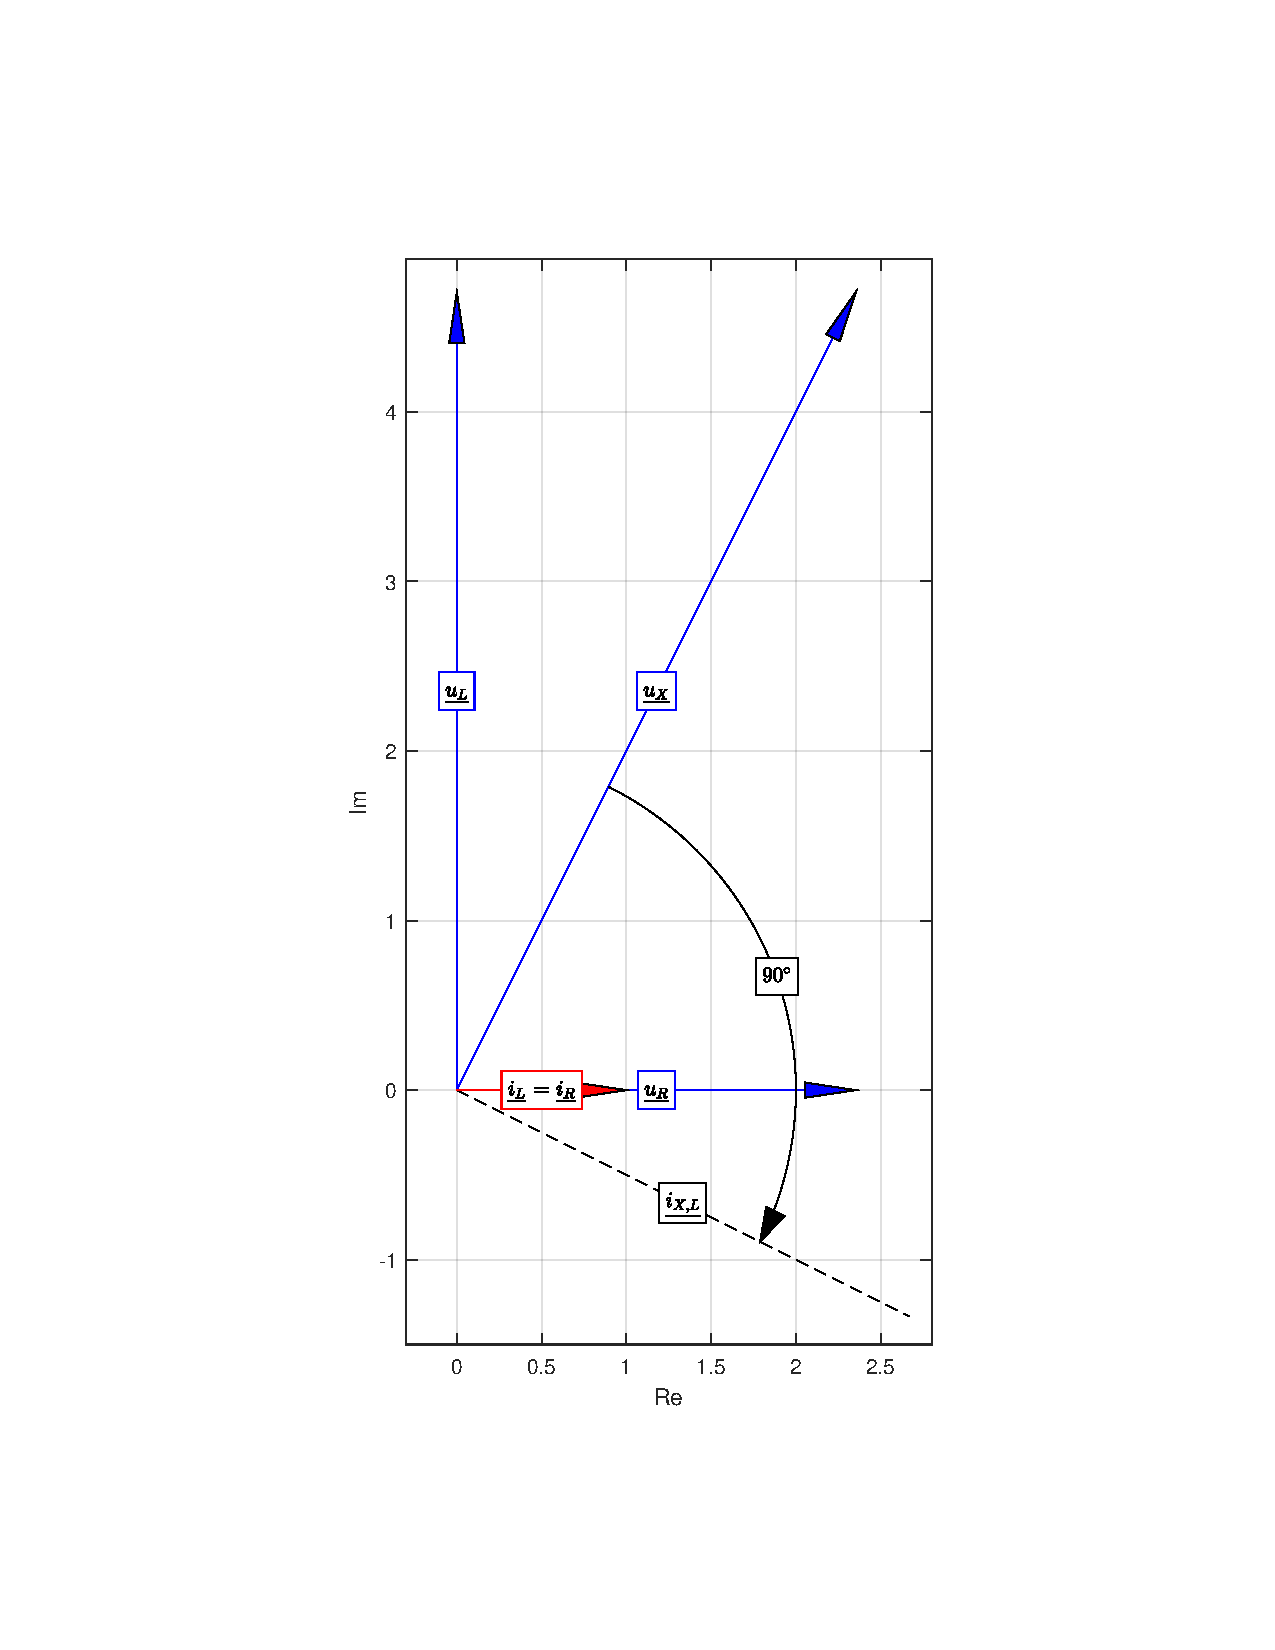
\includegraphics[width=0.45\linewidth]{./Assets/1_L.pdf}
    \caption{Zeigerdiagramm mit Spule als angenommenes Element}
    \label{fig:diagramm-spule}
  \end{center}
\end{figure}


\newpage
\subsection{bei angenommenem Kondensator}
\label{sec:bei-angen-kond}

Die Spannungen wurden wie in Kapitel \ref{sec:skript-zu-kond}, Zeile 52 ersichtlich, mit dem Faktor $1,7$ skaliert. Dies gewährleistet die Darstellung von Strom und Spannung in einem Zeigerdiagramm.

\begin{figure}[!htb]
    \begin{center}
    % \hspace{3cm}
      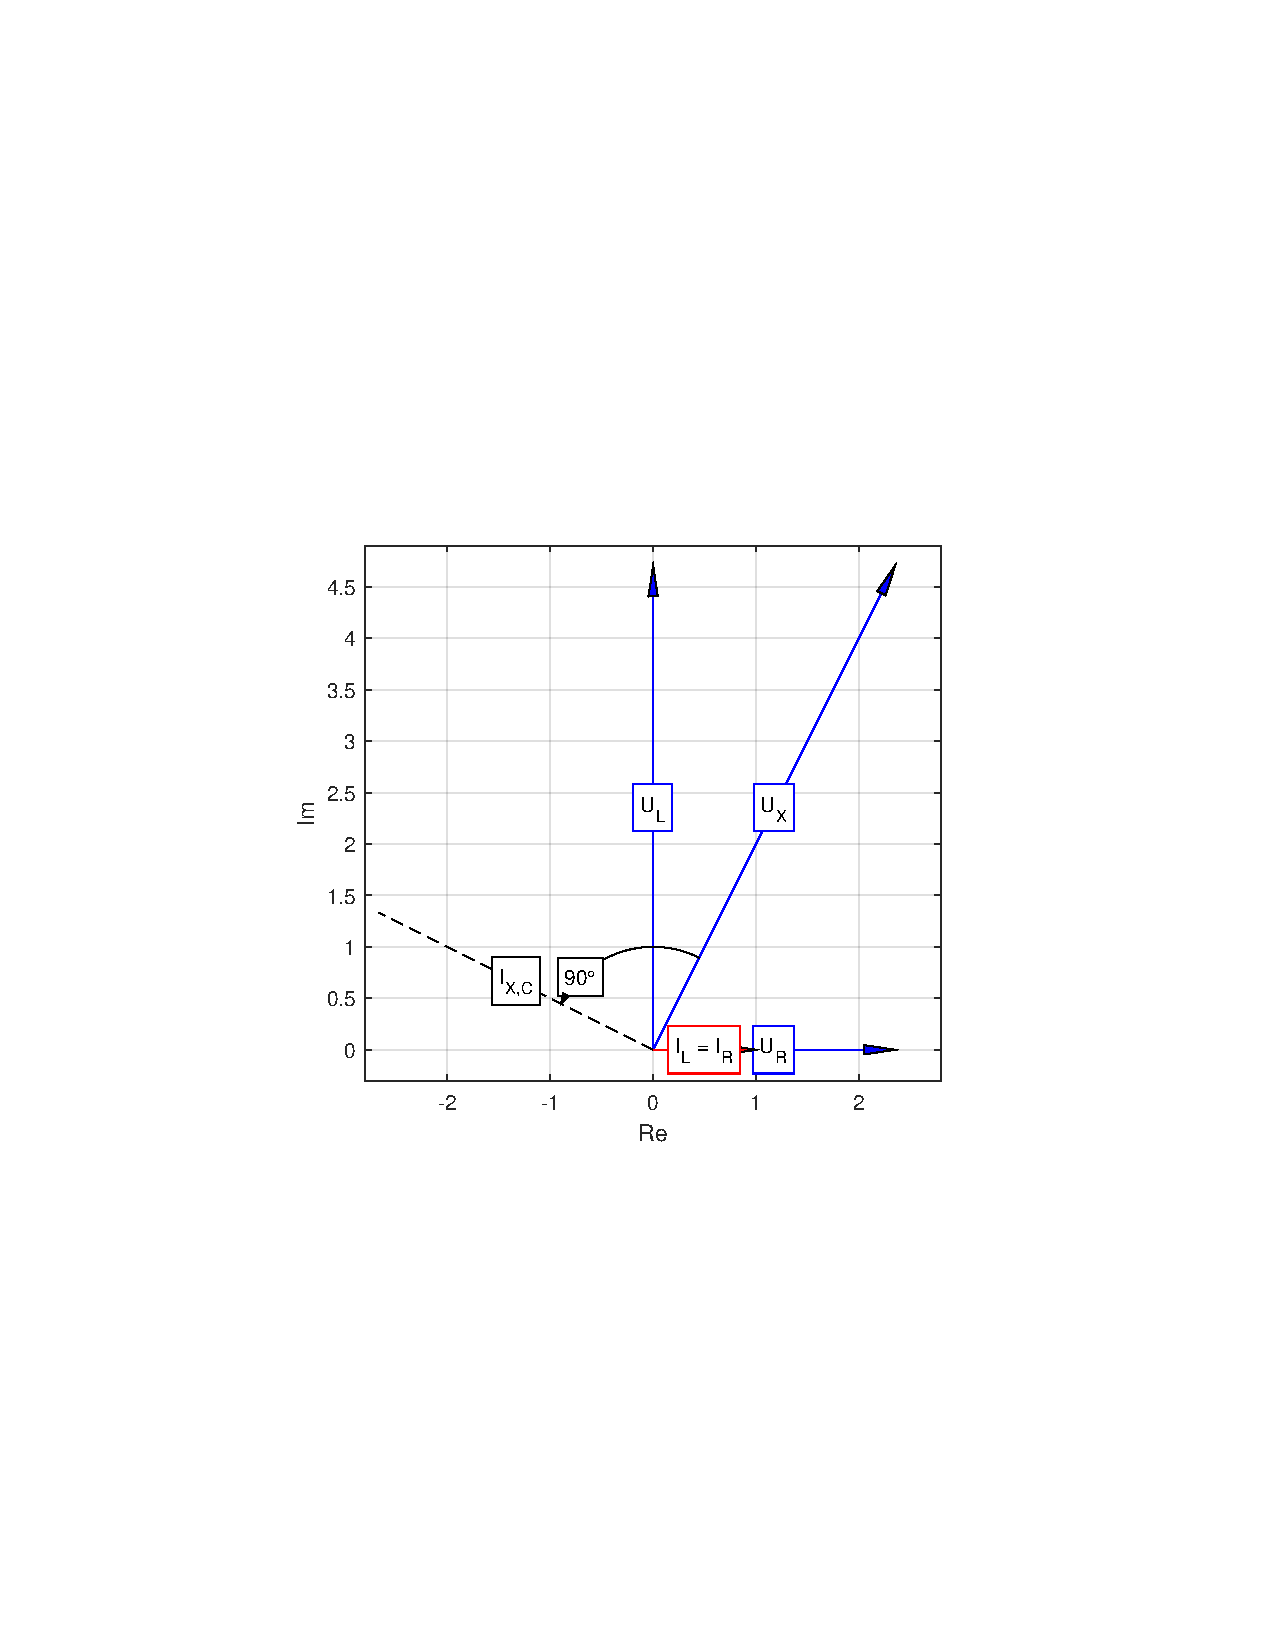
\includegraphics[width=0.90\linewidth]{./Assets/1_C.pdf}
    \caption{Zeigerdiagramm mit Kondensator als unbekanntes Element}
    \label{fig:diagramm-kond}
  \end{center}
\end{figure}



\newpage
\section{Bestimmen der Übertragungsfunktion}
\label{sec:best-der-ubertr}

Um die Bauteile so zu dimensionieren, dass ein Phasenwinkel von $\varphi_{\underline{u_{X}}} = \varphi_{\underline{i_{C}}} + 18,435^{\circ}$ zustande kommt, wird eine Übertragungsfunktion $\underline{F}$ ermittelt.

\begin{equation} \label{eq:uebertrag}
  \underline{u_{x}} = \underline{F} \cdot \underline{i_{C}}
\end{equation}

Um $\underline{F}$ zu erhalten, wird zuerst $\underline{u_{X}}$ mithilfe des ohm'schen Gesetzes ausgedrückt. Da $\underline{i_{X}}$ unbekannt ist, wird jener mittels eines Stromteilers von $\underline{i_{C}}$ ausgedrückt. Durch anschließendes Einsetzen und Umformen lässt sich nun $\underline{u_{X}}$ als Produkt von $\underline{i_{C}}$ mit bekannten Werten ($=\underline{F}$) darstellen.

\begin{align*}
  \underline{u_{X}} &= {\color{red}{\underline{i_{X}}}} \cdot j X_{X} \\
  {\color{red}{\underline{i_{X}}}} &= \underline{i_{C}}\cdot  \frac{R + j X_{L}}{R + j X_{L} + j X_{X}} \\
  \Longrightarrow \underline{u_{X}} &= \underline{i_{C}} \cdot \frac{R + j X_{L}}{R + j (X_{L} + X_{X})} \cdot j X_{X} \\
                    &= \underline{i_{C}} \cdot \frac{-X_{X} \cdot X_{L} + j\cdot R \cdot X_{X}}{R + j (X_{L} + X_{X})} \cdot {\color{orange}{\frac{R-j(X_{L} + X_{X})}{R-j(X_{L} + X_{X})}}} \\
                    &= \underline{i_{C}} \cdot \frac{-X_{X} \cdot X_{L} \cdot R + j \cdot R^{2} \cdot X_{X} + j \cdot X_{X} \cdot X_{L} (X_{L} + X_{X}) + R \cdot X_{X} (X_{L} + X_{X})}{R^{2} + (X_{L} + X_{X})^{2}} \\
                    &= \underline{i_{C}} \cdot \frac{{\color{darkspringgreen}{-X_{X} \cdot X_{L} \cdot R + R \cdot X_{X} \cdot X_{L}}} + R \cdot X_{X}^{2} + j \left( R^{2} \cdot X_{X} + X_{X} \cdot X_{L}^{2} + X_{X}^{2} \cdot X_{L}\right)}{R^{2} + (X_{L} + X_{X})^{2}} \\
                      &= \underline{i_{C}} \cdot \left(\underbrace{\frac{R \cdot X_{X}^{2}}{R^{2} + (X_{L} + X_{X})^{2}}}_{=\operatorname{Re} (\underline{F})} + j \cdot \underbrace{\frac{X_{X} (R^{2} + X_{L}^{2} + X_{X} \cdot X_{L})}{R^{2} + (X_{L} + X_{X})^{2}}}_{=\operatorname{Im} (\underline{F})} \right)
\end{align*}

Da $\underline{i_{C}}$ mit der Übertragungsfunktion $\underline{F}$ multipliziert wird, werden deren Winkel (in der Eulerform) addiert. Somit lässt sich die durch $\underline{F}$ hervorgerufene Phasenverschiebung als \(\arctan\left( \frac{\operatorname{Im}}{\operatorname{Re}}\right)\) ausdrücken. Diese soll dem vorausgesetzten Winkel von $18,435^{\circ}$ entsprechen. Man kann diesen Ausdruck nun nach der gesuchten Größe $X_{X}$ umformen und den Bauteilwert ermitteln.

\begin{align*}
  18,435^{\circ} &\overset{!}{=} \arctan\left(\frac{X_{X} (R^{2} + X_{L}^{2} + X_{X} \cdot X_{L})}{R \cdot X_{X}^{2}}\right) \\
  \tan(18,435^{\circ}) &= \frac{X_{X} (R^{2} + X_{L}^{2} + X_{X} \cdot X_{L})}{R \cdot X_{X}^{2}} \\
  \tan(18,435^{\circ}) \cdot R \cdot X_{X} &= R^{2} + X_{L}^{2} + X_{X} \cdot X_{L} \\
  X_{X} \cdot (\tan(18,435^{\circ})  R - X_{L}) &= R^{2} + X_{L}^{2} \\
  X_{X} &= \frac{R^{2} + X_{L}^{2}}{\tan(18,435^{\circ})  R - X_{L}} \\
                       &= \frac{(4 \unit{$\Omega$})^{2} + (1000 \unit{s}^{-1} \cdot 8 \unit{mH})^{2}}{\tan(18,435^{\circ})  4 \unit{$\Omega$} - (1000 \unit{s}^{-1} \cdot 8 \unit{mH})} \\
                       &= -12 \unit{$\Omega$} \\
  \Longrightarrow X_{X} &= -\frac{1}{\omega \cdot C_{X}} \\
  C_{X} &= -\frac{1}{X_{X} \cdot \omega} = \frac{1}{(-12 \unit{$\Omega$}) \cdot 1000 \unit{s}^{-1}} = 83,33 \unit{$\upmu$F}
\end{align*}

Das negative Vorzeichen bei dem Ergebnis von $X_{X}$ lässt auf einen Kondensator schließen, da dort $X = \frac{1}{\omega C}$.

\section{Bestimmen aller Spannungen und Ströme}
Mithilfe des Teststromes von $\underline{i_{L}} = 1 \unit{A}$ lassen sich sich die Werte aller Ströme und Spannungen der Schaltung folgendermaßen bestimmen:
\begin{align*}
  \underline{Z_{L}} &= j \cdot \omega \cdot L \\
  \underline{Z_{C}} &= \frac{1}{j \cdot \omega \cdot C} \\
  \underline{Z_{C,X}} &= \frac{1}{j \cdot \omega \cdot C_{X}}
\end{align*}

\begin{align*}
  \underline{u_{L}} &= \underline{Z_{L}} \cdot \underline{i_{L}} = (8 \angle 90^{\circ})\unit{V}\\
  \underline{u_{R}} &= R \cdot \underline{i_{L}} = (4 \angle 0^{\circ})\unit{V} \\
  \underline{u_{X}} &= \underline{u_{R}} + \underline{u_{L}} = (8,94 \angle 63,435^{\circ}) \unit{V} \\
  \underline{i_{X}} &= \frac{\underline{u_{X}}}{\underline{Z_{C,X}}} = (0,74 \angle 153,43^{\circ}) \unit{A} \\
  \underline{i_{C}} &= \underline{i_{X}} + \underline{i_{L}} = (0,47 \angle 45^{\circ}) \unit{A} \\
  \underline{u_{C}} &= \underline{i_{C}} \cdot \underline{Z_{C}} = (9,43 \angle -45^{\circ}) \unit{V} \\
  \underline{u_{S}} &= \underline{u_{C}} + \underline{u_{X}} = (10,75 \angle 7,13^{\circ}) \unit{V} \\
\end{align*}

Wie ersichtlich, entspricht der Betrag der Quellspannung $|\underline{u_{S}}|$ nicht den vorgegebenen $10 \unit{V}$. Um dies anzupassen, werden alle Beträge der komplexen Größen mit dem Skalierungsfaktor $\frac{10 \unit{V}}{|\underline{u_{S}}|} = 0,9303$ multipliziert.
Um $\underline{u_{S}}$ abschließend auf die reale Achse zu legen, können alle Werte außerdem um den Phasenwinkel von $\underline{u_{S}}$ im Uhrzeigersinn gedreht werden.
Man erhält nun folgende Werte:

\begin{align*}
  \underline{u_{L}} &= ((8 \cdot 0,9303) \angle( 90^{\circ}- 7,13^{\circ}))\unit{V}  = (7,44 \angle 82,88^{\circ}) \unit{V}\\
  \underline{u_{R}} &= ((4 \cdot 0,9303)\angle( 0^{\circ}- 7,13^{\circ}))\unit{V}  = (3,72 \angle -7,13^{\circ}) \unit{V}\\
  \underline{u_{X}} &= ((8,94 \cdot 0,9303)\angle( 63,435^{\circ}- 7,13^{\circ})) \unit{V} = (8,32 \angle 56,31^{\circ}) \unit{V}\\
  \underline{i_{X}} &= ((0,74 \cdot 0,9303)\angle( 153,43^{\circ}- 7,13^{\circ})) \unit{A} = (0,69 \angle 146,31^{\circ}) \unit{V}\\
  \underline{i_{C}} &= ((0,47 \cdot 0,9303)\angle( 45^{\circ}- 7,13^{\circ})) \unit{A} = (0,44 \angle 37,88^{\circ}) \unit{V}\\
  \underline{u_{C}} &= ((9,43 \cdot 0,9303)\angle( -45^{\circ}- 7,13^{\circ})) \unit{V} = (8,77 \angle -52,13^{\circ}) \unit{V}\\
  \underline{u_{S}} &= ((10,75 \cdot 0,9303)\angle( 7,13^{\circ}- 7,13^{\circ})) \unit{V} = (10 \angle 0^{\circ}) \unit{V}\\
\end{align*}

Mit diesen Werten wurde der Plot in Abbildung \ref{fig:diagramm-kond-bekannt} erstellt.

\newpage
\section{Mögliche Bauteilkombinationen als Lösung}
Beim Bestimmen der Übertragungsfunktion $\underline{F}$ kommt man auf folgenden Wert für $X_{X}$:
\begin{equation}
  \label{eq:2}
  X_{X} = \frac{R^{2} + X_{L}^{2}}{\tan(18,435^{\circ})\cdot R -X_{L}}
\end{equation}

Da der Nenner nicht Null werden darf, lässt sich folgendes Verhältnis von $X_{L}$ zu $R$ ausschließen:
\begin{align*}
  \frac{X_{L}}{R} = \tan(18,435^{\circ})
\end{align*}

Der Zähler des Bruchs in Formel \ref{eq:2} kann nicht negativ werden. Das Vorzeichen des Bruchs entscheidet jedoch, ob es sich um eine Spule (positiver Wert) oder einen Kondensator (negativer Wert) handelt. Somit gilt:
\begin{align*}
  \tan(18,435^{\circ})\cdot R -X_{L}
  \begin{cases}
    < 0 & \Longrightarrow \text{Kondensator}\\
    > 0 & \Longrightarrow \text{Spule}
  \end{cases}
\end{align*}

\newpage
\section{Matlab-Plots}
\label{sec:matlab-skripten}
\subsection{Zeigerdiagramm mit Kondensator als nun bekanntes Element}
\label{sec:zeig-mit-kond-bekannt}

Die Spannungen wurden wie in Kapitel \ref{sec:skript-zu-kond-1}, Zeile 62 ersichtlich, mit dem Faktor $9$ skaliert. Dies gewährleistet die Darstellung von Strom und Spannung in einem Zeigerdiagramm.

\begin{figure}[!htb]
    \begin{center}
    % \hspace{3cm}
      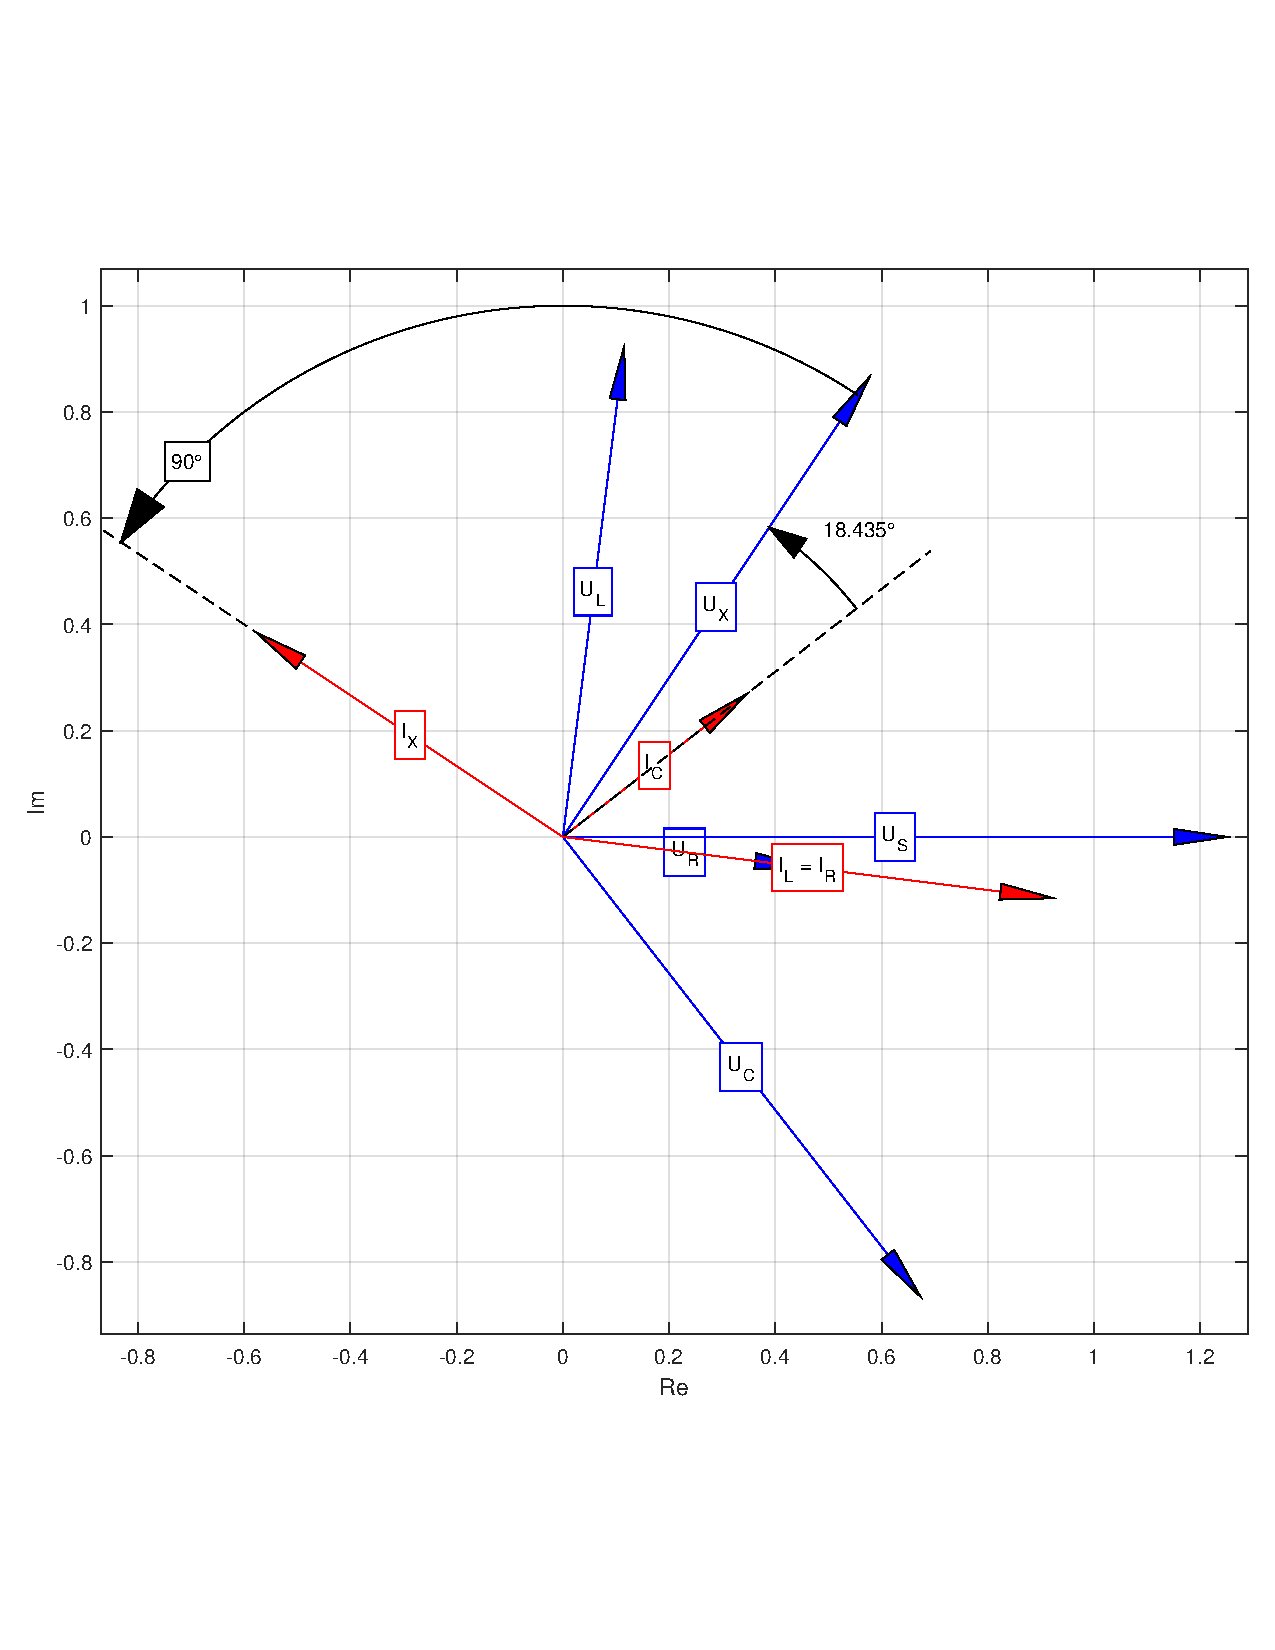
\includegraphics[width=0.9\linewidth]{./Assets/gesamt_TEST.pdf}
    \caption{Zeigerdiagramm mit Kondensator als nun bekanntes Element}
    \label{fig:diagramm-kond-bekannt}
  \end{center}
\end{figure}



\newpage
\section{Matlab-Skripten}
\label{sec:matlab-skripten-1}

\subsection{Skript zu Kondensator als unbekanntes Element}
\label{sec:skript-zu-kond}
\lstinputlisting[language=Matlab]{./Assets/Kond.m}


\subsection{Skript zu Spule als unbekanntes Element}
\label{sec:skript-zu-spule}
\lstinputlisting[language=Matlab]{./Assets/Spule.m}


\subsection{Skript zu Kondensator als nun bekanntes Element}
\label{sec:skript-zu-kond-1}
\lstinputlisting[language=Matlab]{./Assets/Gesamt.m}

\newpage
\section{PSpice-Simulation}
\label{sec:pspice-simulation}

\subsection{Schaltbild}
\label{sec:schaltbild}

\begin{figure}[!htb]
    \begin{center}
    % \hspace{3cm}
      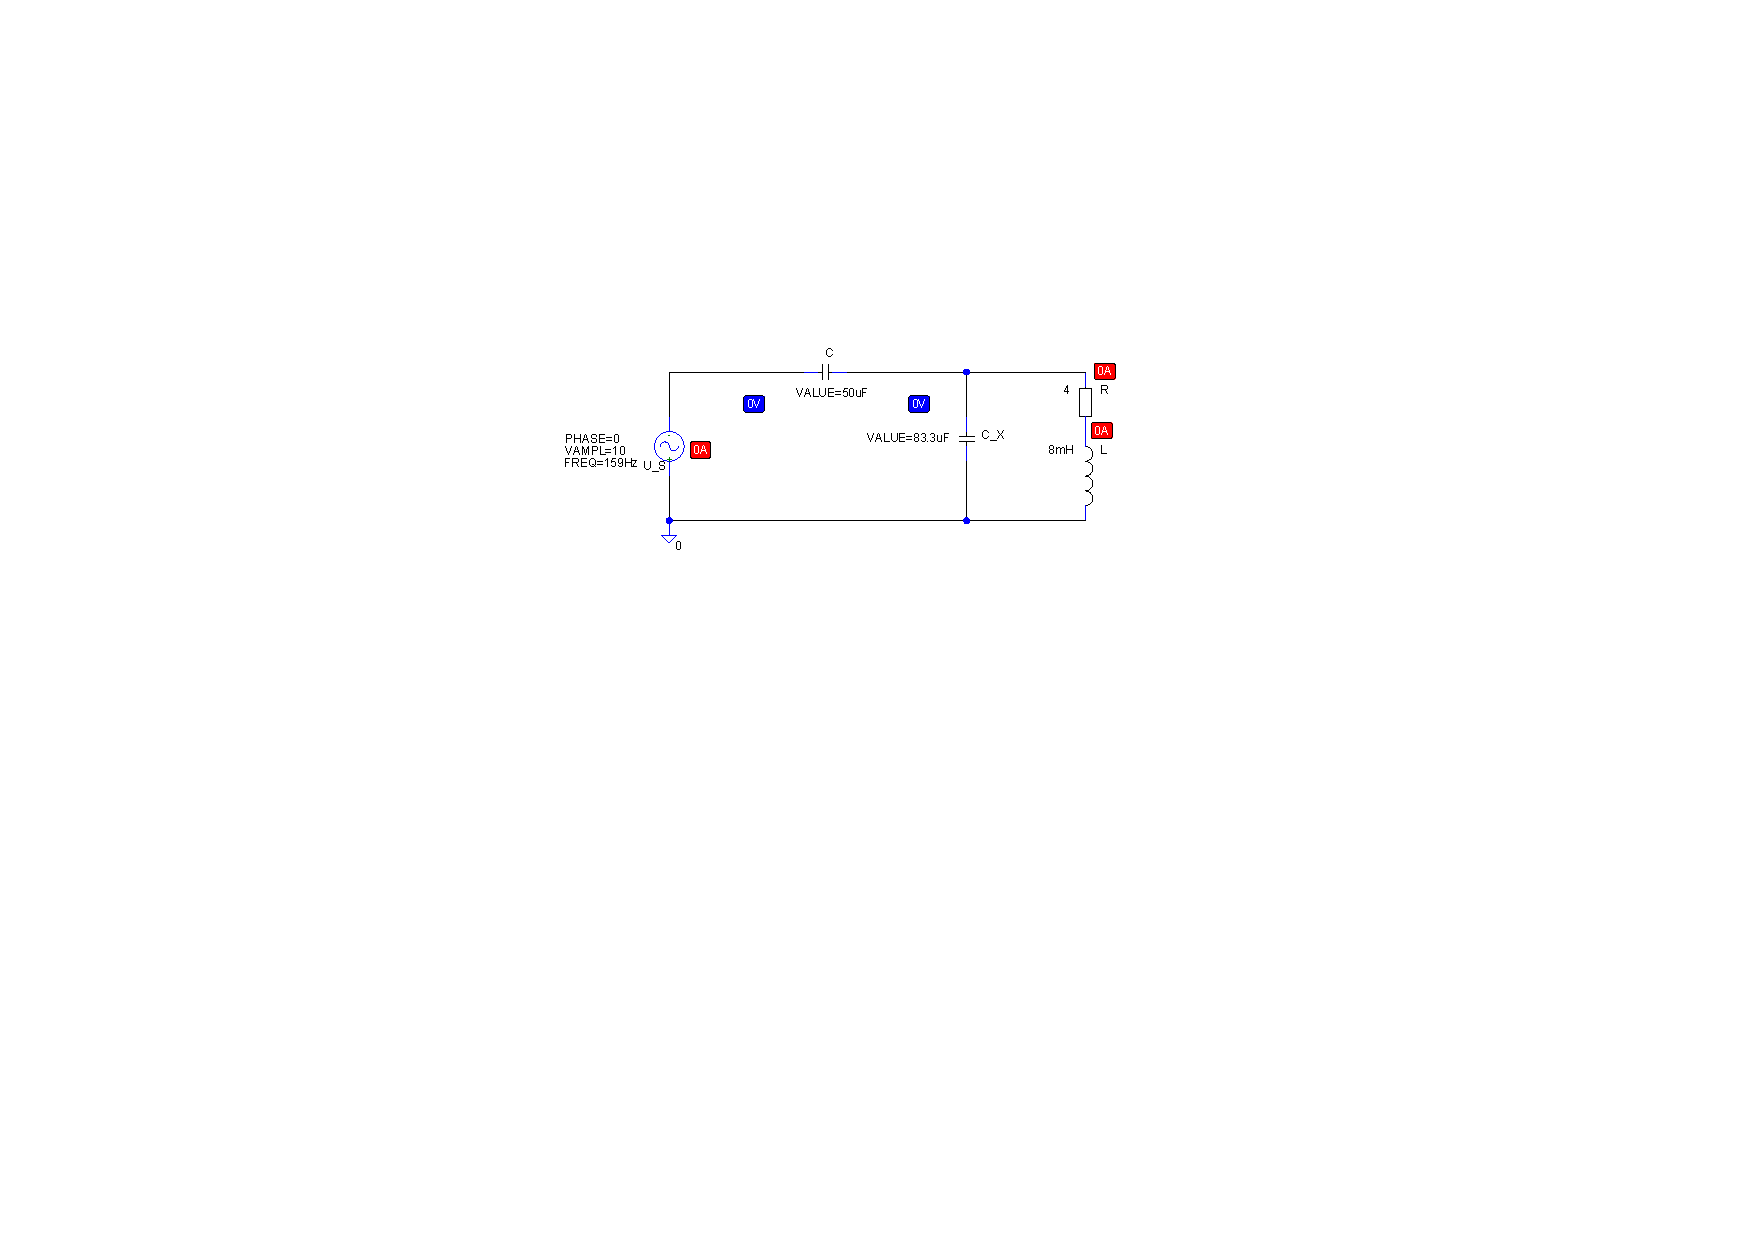
\includegraphics[width=0.9\linewidth]{./Assets/PS_Schaltplan.pdf}
    \caption{Schaltbild der zu simulierenden Schaltung}
    \label{fig:schaltbild}
  \end{center}
\end{figure}


\subsection{Plot}
\label{sec:plot}

\begin{figure}[!htb]
    \begin{center}
    % \hspace{3cm}
      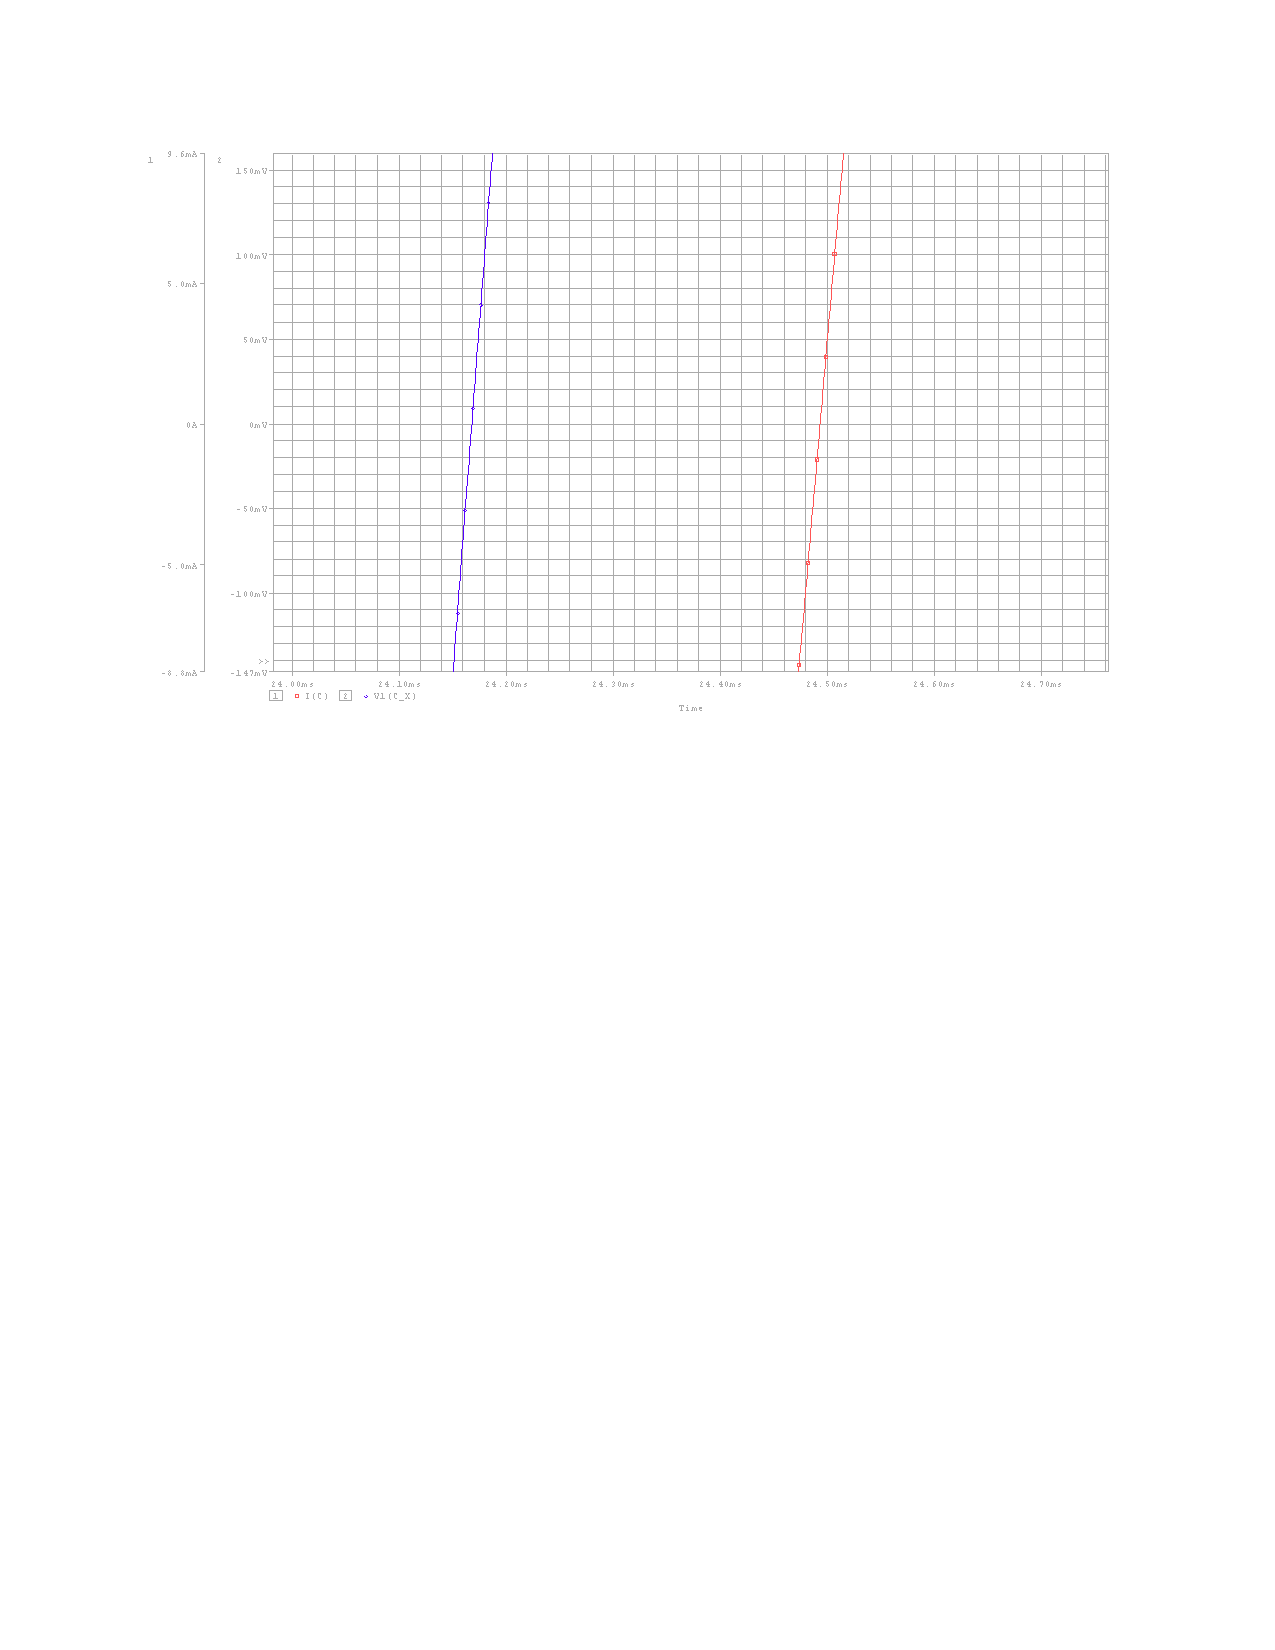
\includegraphics[width=\linewidth]{./Assets/PS_Plot.pdf}
    \caption{Ausschnitt des Simulationsplots der beiden Größen $u_{C,X}$ und $i_{C}$}
    \label{fig:simulation}
  \end{center}
\end{figure}

In Abbildung \ref{fig:simulation} lässt sich eine zeitliche Verschiebung von $\underline{i_{C}}$ zu $\underline{u_{C,X}}$ von $\Delta t = 325 \unit{$\upmu$s}$ messen.
Dies entspricht einem Winkel von $\varphi = \frac{\Delta t}{T} \cdot 360^{\circ} = 18,603^{\circ}$. Dem Unterschied von $0,168^{\circ}$ zum vorgegebenen Wert liegen Mess- und Rundungsfehler zugrunde.

\end{document}
